\documentclass[12pt,letterpaper]{article}
\usepackage[utf8]{inputenc}
\usepackage{float}
\usepackage{pdflscape}
\usepackage{amsmath}
\usepackage{amsfonts}
\usepackage{amssymb}
\usepackage{fullpage}
\usepackage{gensymb, comment}
\usepackage{textcomp}
\usepackage{threeparttable}
\usepackage{graphicx}
\usepackage{natbib}
\usepackage{setspace} 
\doublespacing
\usepackage{indentfirst}
\setlength{\parindent}{25pt}
\usepackage{bbm}
\usepackage{multicol}
\usepackage{makecell}
\usepackage{booktabs}
\newtheorem{prop}{Proposition} 
\newtheorem{assumption}{Assumption} 
\newtheorem{implication}{Implication} 
\usepackage{longtable}

\setcounter{totalnumber}{8}

\title{Winter weather on exam days and admission for a prestigious university in Japan}%: \\ Empirical analysis on auditing reports in Brazil}
%\author{Mizuhiro Suzuki\thanks{Department of Agricultural and Applied Economics, University of Wisconsin-Madison. Contact: msuzuki7@wisc.edu. The authors would like to thank Laura Schechter for her numerous feedback and support. We are also grateful to Joshua Deutschmann, Paul Dower, Jeremy Foltz, Priya Mukherjee, Andrew Stevens, and seminar participants at the UW-Madison Agricultural and Applied Economics department for helpful comments and suggestions. Any errors in this draft are the sole responsibility of the authors.}}
\author{Mizuhiro Suzuki\thanks{Department of Agricultural and Applied Economics, University of Wisconsin-Madison. Contact: msuzuki7@wisc.edu}}
\date{\today \\ \vspace{1cm} Preliminary draft \\ Please do not cite or circulate}

\begin{document}
  
\maketitle
\begin{abstract}
  \singlespacing
     \noindent 
  
  \medskip
  \vspace{1cm}
 \noindent Keywords: Temperature, Education, University admission, Cognitive performance
\end{abstract}

\newpage

\section{Introduction}

External factors can impact various outcomes.
One active area of research is the effect of high temperature on performance at high-stakes exams.
Given the importance of high education for later outcomes, this is nice.

What is missing in the literature is the effect of \textit{low} temperature on performance at exams.

In this study, I analyze the effect of winter weathers on exam outcomes in Japan.
I use the weather on the days of National Center Test for University Admission (Center Test hereafter) and investigate its effect on the admission for the most prestigious university in Japan, the University of Tokyo (UTokyo henceforth).

If I use a middle-ranked university, reduction in admission share can be attributed to both lower and higher scores:
while students with lower scores can fail to get into the university, students with higher scores can choose to apply to and get admitted to higher-ranked universities.
Since UTokyo is the most prestigious university in Japan (** cite some university ranking **), it is unlikely that students who get high scores in Center Test go to better universities.\footnote{
  Medical departments in several universities are higher-ranked than UTokyo based on standard score.
  However, the career paths for those in the non-medical department of UTokyo and medical departments in universities are substantially different:
  while most students graduating from medical departments become medical doctors, the majority of students from UTokyo become bureaucrats, work for private firms, or go to graduate schools.
  Hence, it is unlikely that high scores at Center Test induce students who would otherwise get into UTokyo to go to a medical department.
}
Therefore, if I observe a reduction in admission share, I consider this as an evidence that the performance in Center Test is negatively affected. 

\section{Background}

For admission for most (especially almost all public) universities, students are required to take two exams.
The first stage is Center Test.
Students take an exam on consecutive two days (Saturday and Sunday on mid January).
While different students can choose which subjects to take, most universities require students to take exams on math, English, language, natural science, and social science.
Questions are multiple-choice and common for all exam takers across Japan.
Exam takers do not receive their exact scores until the next May at earliest.
However, since they can record their answers to the exam booklets and can bring them back home, they know their scores by comparing their own answers and correct answers, which are made public through newspaper or websites of cramming schools.
High-school seniors take the test at designated cites in the area where their high schools are located.
On the other hand, high-school graduates are assigned to test cites in the area where the homes used in their application forms are located.

After taking Center Test, students apply for public and private universities.\footnote{
  There are private universities who accept applications before Center Test.
}
Applicants for public universities typically take the second-stage exam.
This exam is made by each university, and students go to the universities and take the exam.
In other words, every applicant for a university takes the exam at the same location.

For public universities, there are three exam periods: the first one is typically at the end of February, the second one is on the first week of March, and the third one is typically around March 10th.
While different universities accept applications for different periods, most universities have only one (typically the first period) or two (typically the first and the third periods) periods.
UTokyo has two exam periods, the first and the third ones, although most of the admissions are provided for exam takers during the first exam period.

For UTokyo, scores at Center Test are used for two purposes.
First, the scores are used for eligibility to take the second-stage exam.
Thresholds varying across years and across majors are set, and if scores at Center Test are below the thresholds, students cannot take the second-stage exam.
Since the thresholds are announced after the application, exam takers do not know if their scores are above or below the thresholds. 

Secondly, the scores at Center Test are taken into consideration for admission.
The final score of a students is calculated by the weighted average of exam scores at the first- and second-stage exams.

\section{Data}

I use two sets of data: weather and admission information for UTokyo.
For weather information, I get data from Japan Meteorological Agency.
Their website maintains the past weather across Japan.
In this study, based on hourly weather on exam days at prefecture capitals, I use average weathers between 6AM to 6PM.
Prefecture capitals tend to be most populated in each prefecture, and in many prefectures highly-ranked high schools from which many students go to UTokyo are located at prefecture capitals.
%\footnote{
%  According to inter-edu, \url{https://www.inter-edu.com/univ/2019/jisseki/todai/ranking/}
%}

For admission information for UTokyo, I use University Basic Information maintained by National Institution for Academic Degrees and Quality Enhancement of Higher Education.
This data contains information from 2012 to 2020 on the number of admitted students by prefectures at which their high schools are located.
I create the admission share of each prefecture, which is the ratio of the number of admitted students from a prefecture to the number of all admitted students.

The summary statistics are provided in Table \ref{tab:sum_stat}.
While the mean of the admission share (\%) is $2.08$,\footnote{
  Since there are admissions from abroad, the mean value does not coincide with $1 / 47 \approx 2.12\%$.
} the distribution is starkly skewed.
As shown in Figure \ref{fig:admission_map}, many prefecture have less 1\% shares.
Also, the admission shares of the top 5 prefectures total more than 60\%.
This results in a small median admission share, $0.79$.

\begin{table}[H]
  \centering
  \caption{Summary Statistics}
  \resizebox{\linewidth}{!}{
  
\begin{tabular}[t]{lllllll}
\toprule
\multicolumn{1}{c}{ } & \multicolumn{1}{c}{N} & \multicolumn{1}{c}{Mean} & \multicolumn{1}{c}{SD} & \multicolumn{1}{c}{Median} & \multicolumn{1}{c}{Min} & \multicolumn{1}{c}{Max} \\
\cmidrule(l{3pt}r{3pt}){2-2} \cmidrule(l{3pt}r{3pt}){3-3} \cmidrule(l{3pt}r{3pt}){4-4} \cmidrule(l{3pt}r{3pt}){5-5} \cmidrule(l{3pt}r{3pt}){6-6} \cmidrule(l{3pt}r{3pt}){7-7}
Matriculation share (\%) & 423 & 2.08 & 5.23 & 0.79 & 0.06 & 37.35\\
Temperature (\degree C) & 423 & 4.67 & 3.81 & 4.98 & -6.63 & 19.86\\
Hourly precipitation (mm) & 423 & 0.08 & 0.18 & 0.00 & 0.00 & 1.27\\
Hourly snowfall (m) & 423 & 0.00 & 0.00 & 0.00 & 0.00 & 0.01\\
Cumulated snow (m) & 423 & 0.05 & 0.15 & 0.00 & 0.00 & 1.26\\
\bottomrule
\end{tabular}

  }
  \label{tab:sum_stat}
  \footnotesize
  \begin{tablenotes}
    \item 
      Notes:
      Admission share (\%) is the share of newly admitted students to the University of Tokyo from each prefecture.
      The admission share is calculated based on the ratio of the number of students from high schools in the prefecture to the total number of admission.
      I use weather variables at prefecture capitals between 6AM and 6PM on days of Center Test.
  \end{tablenotes}
\end{table}

\begin{figure}[H]
  \centering
  \caption{Map of admission shares (\%) (average across years)}
  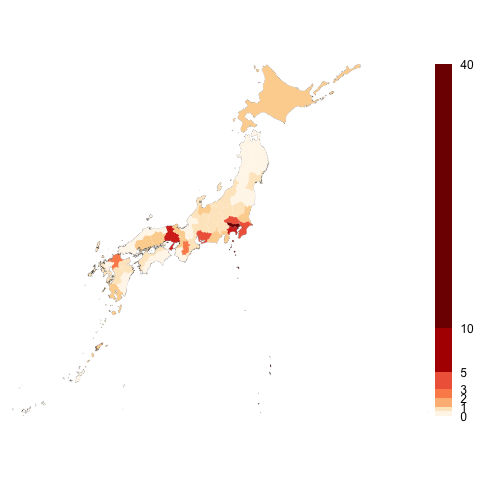
\includegraphics[width = 0.9\textwidth]{../Output/images/admission_map.png}
  \label{fig:admission_map}
  \footnotesize
  \begin{tablenotes}
    \item Notes:
      This map shows the admission shares (\%) for the University of Tokyo from each prefecture.
      The admission share is calculated based on the ratio of the number of students from high schools in the prefecture to the total number of admission.
      Average of the shares across years is shown in the map.
      Although not shown in the legend due to the lack of the space, the lightest color in the map means the admission share between 0 to 0.5\% 
  \end{tablenotes}
\end{figure}

\section{Empirical Strategy}

The objective of the analysis is to analyze the effect of temperature and other weather variables on exam days on the admission share for UTokyo.
The outcome variable, $Y_{jt}$ is the admission share (\%) for UTokyo of a prefecture $j$ in year $t$.
Let $T_{jt}$ be average temperature on exam days in $j$ in year $t$.
I use functions of $T_{jt}$ in the regressions ($f$), which can be linear or non-linear.
I include other weather variables such as rainfall, snowfall, and cumulated snow on exam days as a vector $X_{jt}$.
As fixed effects, prefecture fixed effects ($\mu_j$) and year fixed effects ($\tau_t$) are used.
Finally, the error term is represented as $\epsilon_{jt}$.

I run the following regression equation:
\begin{equation*}
  Y_{jt} = f(T_{jt}) + X_{jt}' \beta + \mu_j + \tau_t + \epsilon_{jt}.
\end{equation*}
I exploit the variation of temperature on exam days, which I consider exogenous after controlling for prefecture-specific time-variant factors and time-varying aggregate shocks through prefecture and year fixed effects.
As Figure \ref{fig:temperature_diff} shows, each prefecture experiences substantial variation in temperature on exam days.\footnote{
  Similar figures for other weather variables are provided in Appendix \ref{sec:appendix_figure}.
}

One potential problem in the analysis is that a students from a high school in a prefecture does not necessarily take Center Test in the same municipality.
This means that, for these students, the weather at the exam cites are measured with errors.
The primary reason for this to happen is that a senior student at a high school located at a prefecture different from his home prefecture fails to get in any university for the first year and retake Center Test next year in his home prefecture.
I consider that, conditional on prefecture fixed effects, the measurement error is likely to be uncorrelated with the error term.
Hence, this classical measurement error can make the estimates conservative.

\begin{figure}[H]
  \centering
  \caption{Average temperature on two exam days in each prefecture each year}
  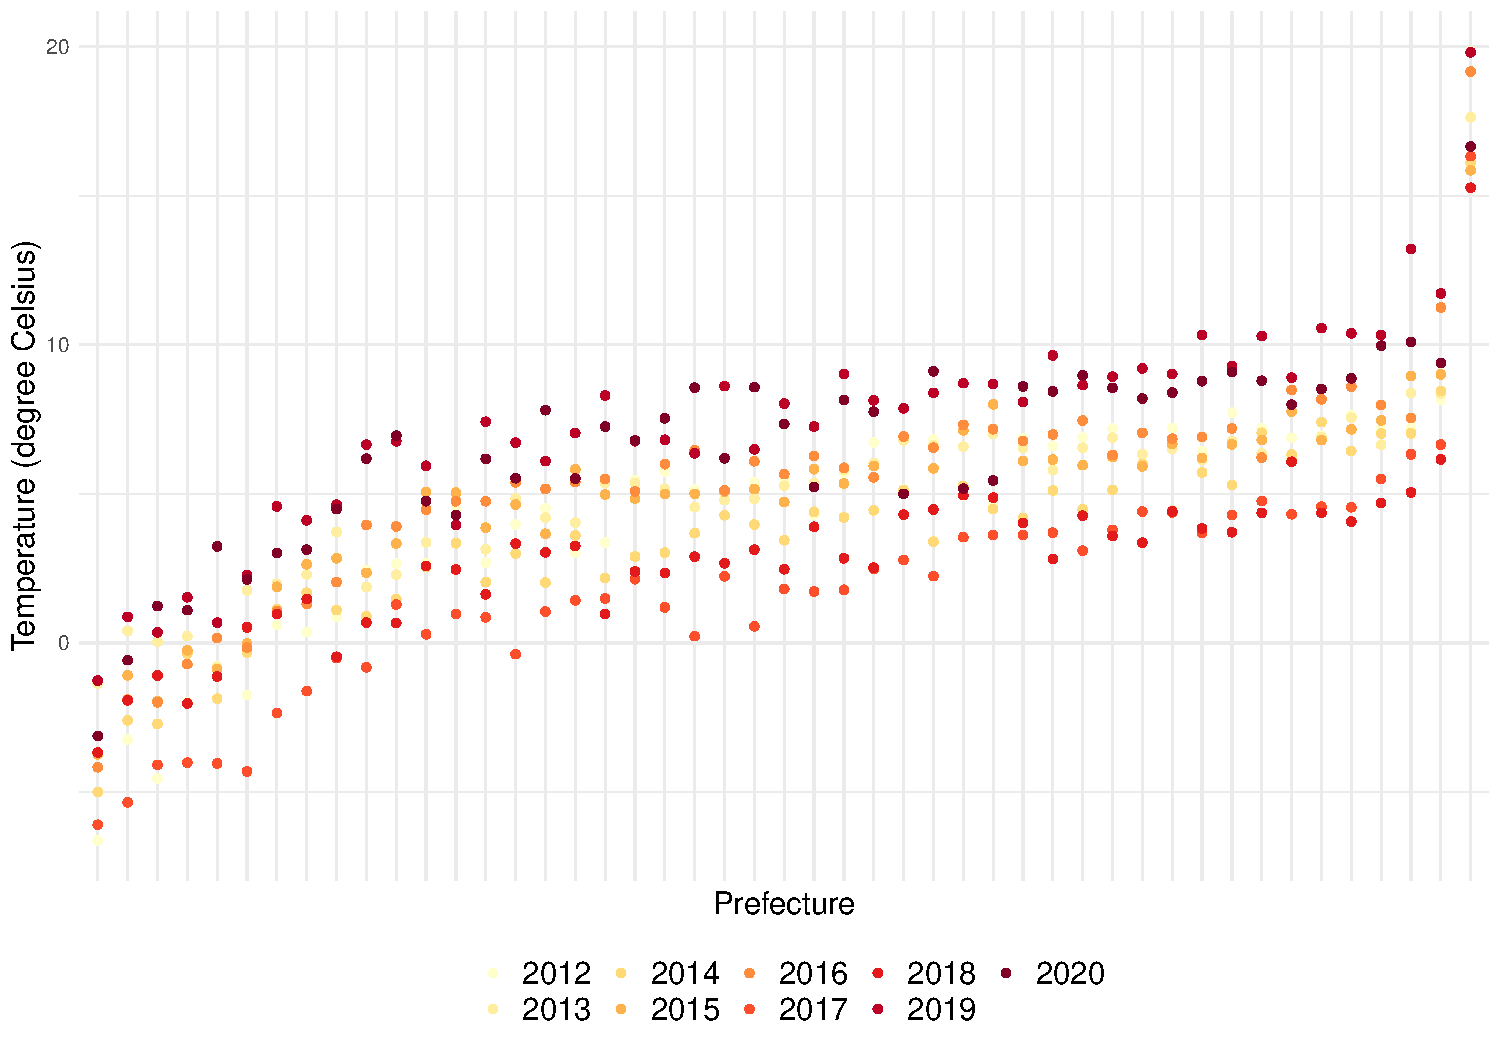
\includegraphics[width = 0.9\textwidth]{../Output/images/temperature_diff.pdf}
  \label{fig:temperature_diff}
  \footnotesize
  \begin{tablenotes}
    \item Notes:
      Temperature at prefecture capitals between 6AM and 6PM on days of Center Test is used.
      Average across two test days in each year is shown in the figure.
      Prefectures positioned to the left on the x-axis are located at more northern parts of Japan.
  \end{tablenotes}
\end{figure}

\section{Results}

\subsection{Main Results}

The main empirical results are provided in Table \ref{tab:main_reg}.
The column (1) shows the result with a linear specification.
While the point estimate is positive, which means admission shares are higher if an exam is held on warmer days, it is statistically insignificant. 
The estimates with a non-linear specification allowing for flexible temperature effects (column (2)) show a negative and statistically significant impacts of cold weather. 
Since the mean admission share is $2.08$\%, the coefficient on the lowest temperature bins means that reducing the temperature from the reference bin (between 3 and 6 $^o$C) to the lowest bin, the admission share decreases by 9\%.
Moreover, due to the stark skewness in the distribution of admission shares, the median admission share is $0.79$.
Therefore, the same temperature change decreases the admission share by 22\% of the median value.
Also, the plateau effect of temperature above 6 $^o$C could be the reason why the linear specification in the column (1) could not capture the non-linear effect of temperature and why the coefficient is statistically insignificant.
Although for a quite different temperature range, similar plateau effects are found in Park (2020) and Melo and Suzuki (2021).

In column (3) and (4), I add other weather variables.
While temperature coefficients are barely affected, I find that rainfall and snowfall during exam time do not impact the admission shares.
On the other hand, the cumulated snow on the ground has a negative impact.
To capture the effect of existence of snow on the ground, column (5) allows a non-linear effect of cumulated snow.
This specification gives a result that, when there is snow on the ground cumulated more than 10cm ($\approx$ 3 feet) decreases the admission share by 0.13 percentage point.

In summary, I find a both statistically and economically significant impacts of weather on exam days.
In particular, the estimation results show that low temperature and snow cumulated on the ground have negative impact on the admission shares for UTokyo.
In the next two subsections, I investigate the mechanisms underlying the findings. 

\begin{table}[H]
  \center
  \caption{Regression: Admission share (\%) and weather on exam days}
  
% Table created by stargazer v.5.2.2 by Marek Hlavac, Harvard University. E-mail: hlavac at fas.harvard.edu
% Date and time: Tue, May 04, 2021 - 11:24:34
\begin{tabular}{@{\extracolsep{5pt}}lcccc} 
\\[-1.8ex]\hline 
\hline \\[-1.8ex] 
 & \multicolumn{4}{c}{\textit{Dependent variable:}} \\ 
\cline{2-5} 
\\[-1.8ex] & \multicolumn{4}{c}{Matriculation share (\%)} \\ 
\\[-1.8ex] & (1) & (2) & (3) & (4)\\ 
\hline \\[-1.8ex] 
 Temperature (\degree C) $\le$ 0 & $-$0.18$^{**}$ & $-$0.19$^{**}$ & $-$0.16$^{**}$ & $-$0.15$^{*}$ \\ 
  & (0.08) & (0.08) & (0.08) & (0.08) \\ 
  & & & & \\ 
 Temperature (\degree C) 0-3 & $-$0.08$^{*}$ & $-$0.08$^{*}$ & $-$0.08$^{*}$ & $-$0.08$^{*}$ \\ 
  & (0.04) & (0.04) & (0.04) & (0.04) \\ 
  & & & & \\ 
 Temperature (\degree C) 6-9 & 0.13 & 0.13 & 0.13 & 0.13 \\ 
  & (0.10) & (0.09) & (0.09) & (0.09) \\ 
  & & & & \\ 
 Temperature (\degree C) $>$ 9 & 0.14 & 0.14 & 0.15 & 0.15 \\ 
  & (0.12) & (0.12) & (0.12) & (0.12) \\ 
  & & & & \\ 
 Rainfall (mm) &  & $-$0.02 & 0.06 & 0.06 \\ 
  &  & (0.09) & (0.08) & (0.08) \\ 
  & & & & \\ 
 Snowfall (m) &  & 7.75 &  &  \\ 
  &  & (9.95) &  &  \\ 
  & & & & \\ 
 Cumulated snow (m) &  &  & $-$0.19$^{**}$ &  \\ 
  &  &  & (0.09) &  \\ 
  & & & & \\ 
 Cumulated snow $>$ .10 m &  &  &  & $-$0.11$^{***}$ \\ 
  &  &  &  & (0.04) \\ 
  & & & & \\ 
\hline \\[-1.8ex] 
Prefecture FE & Yes & Yes & Yes & Yes \\ 
Year FE & Yes & Yes & Yes & Yes \\ 
Observations & 423 & 423 & 423 & 423 \\ 
\hline 
\hline \\[-1.8ex] 
\textit{Note:}  & \multicolumn{4}{r}{$^{*}$p$<$0.1; $^{**}$p$<$0.05; $^{***}$p$<$0.01} \\ 
\end{tabular} 

  \label{tab:main_reg}
  \small
  \begin{tablenotes}
    \item
      The outcome variable is the admission shares (\%) for the University of Tokyo from each prefecture.
      The admission share is calculated based on the ratio of the number of students from high schools in the prefecture to the total number of admission.
      I use weather variables at prefecture capitals between 6AM and 6PM on days of Center Test.
      Standard errors are clustered at the prefecture level.
  \end{tablenotes}
\end{table}

\subsection{Weather in the morning vs. during exam}

\begin{table}[H]
  \center
  \caption{Regression: Admission share (\%) and weather in the morning vs. during exam}
  \scriptsize
  
% Table created by stargazer v.5.2.2 by Marek Hlavac, Harvard University. E-mail: hlavac at fas.harvard.edu
% Date and time: Tue, Apr 06, 2021 - 10:28:53
\begin{tabular}{@{\extracolsep{5pt}}lcccccc} 
\\[-1.8ex]\hline 
\hline \\[-1.8ex] 
 & \multicolumn{6}{c}{\textit{Dependent variable:}} \\ 
\cline{2-7} 
\\[-1.8ex] & \multicolumn{6}{c}{Matriculation share (\%)} \\ 
\\[-1.8ex] & (1) & (2) & (3) & (4) & (5) & (6)\\ 
\hline \\[-1.8ex] 
 Temperature (morning) $\le$ -3 & $-$0.13$^{**}$ & $-$0.13$^{**}$ &  &  & $-$0.12$^{**}$ & $-$0.13$^{**}$ \\ 
  & (0.06) & (0.06) &  &  & (0.06) & (0.06) \\ 
  & & & & & & \\ 
 Temperature (morning) $>$ -3, $\le$ 0 & $-$0.13$^{***}$ & $-$0.12$^{***}$ &  &  & $-$0.12$^{***}$ & $-$0.12$^{***}$ \\ 
  & (0.04) & (0.04) &  &  & (0.05) & (0.04) \\ 
  & & & & & & \\ 
 Temperature (morning) $>$ 3, $\le$ 6 & 0.004 & 0.01 &  &  & $-$0.01 & $-$0.01 \\ 
  & (0.03) & (0.03) &  &  & (0.04) & (0.04) \\ 
  & & & & & & \\ 
 Temperature (morning) $>$ 6 & $-$0.04 & $-$0.04 &  &  & $-$0.06 & $-$0.06 \\ 
  & (0.06) & (0.06) &  &  & (0.07) & (0.07) \\ 
  & & & & & & \\ 
 Temperature (during-exam) $\le$ 0 &  &  & $-$0.21$^{*}$ & $-$0.18 & $-$0.14 & $-$0.11 \\ 
  &  &  & (0.12) & (0.12) & (0.13) & (0.13) \\ 
  & & & & & & \\ 
 Temperature (during-exam) $>$ 0, $\le$ 3 &  &  & $-$0.12 & $-$0.11 & $-$0.08 & $-$0.07 \\ 
  &  &  & (0.08) & (0.08) & (0.09) & (0.09) \\ 
  & & & & & & \\ 
 Temperature (during-exam) $>$ 6, $\le$ 9 &  &  & $-$0.11 & $-$0.11 & $-$0.10 & $-$0.10 \\ 
  &  &  & (0.08) & (0.08) & (0.08) & (0.09) \\ 
  & & & & & & \\ 
 Temperature (during-exam) $>$ 9 &  &  & $-$0.001 & 0.01 & 0.01 & 0.02 \\ 
  &  &  & (0.06) & (0.05) & (0.06) & (0.06) \\ 
  & & & & & & \\ 
 Rainfall (mm) (morning) & $-$0.03 & 0.0000 &  &  & 0.01 & 0.02 \\ 
  & (0.07) & (0.06) &  &  & (0.07) & (0.06) \\ 
  & & & & & & \\ 
 Snowfall (m) (morning) & 1.52 &  &  &  & $-$0.14 &  \\ 
  & (6.97) &  &  &  & (7.62) &  \\ 
  & & & & & & \\ 
 Cumulated snow (m) (morning) &  & $-$0.15$^{**}$ &  &  &  & $-$0.60 \\ 
  &  & (0.07) &  &  &  & (1.17) \\ 
  & & & & & & \\ 
 Rainfall (mm) (during-exam) &  &  & $-$0.02 & 0.04 & $-$0.03 & 0.002 \\ 
  &  &  & (0.07) & (0.06) & (0.07) & (0.07) \\ 
  & & & & & & \\ 
 Snowfall (m) (during-exam) &  &  & 4.89 &  & 4.25 &  \\ 
  &  &  & (7.20) &  & (7.75) &  \\ 
  & & & & & & \\ 
 Cumulated snow (m) (during-exam) &  &  &  & $-$0.19$^{**}$ &  & 0.43 \\ 
  &  &  &  & (0.09) &  & (1.16) \\ 
  & & & & & & \\ 
\hline \\[-1.8ex] 
Prefecture FE & Yes & Yes & Yes & Yes & Yes & Yes \\ 
Year FE & Yes & Yes & Yes & Yes & Yes & Yes \\ 
Observations & 423 & 423 & 423 & 423 & 423 & 423 \\ 
\hline 
\hline \\[-1.8ex] 
\textit{Note:}  & \multicolumn{6}{r}{$^{*}$p$<$0.1; $^{**}$p$<$0.05; $^{***}$p$<$0.01} \\ 
\end{tabular} 

  \label{tab:reg_morning_exam}
  \scriptsize
  \begin{tablenotes}
    \item
      The outcome variable is the admission shares (\%) for the University of Tokyo from each prefecture.
      The admission share is calculated based on the ratio of the number of students from high schools in the prefecture to the total number of admission.
      For variables in the morning, I use average weather variables at prefecture capitals between 6AM to 9AM on exam days.
      For variables during the exam, I use average weather variables at prefecture capitals between 9AM to 6PM on exam days.
      Standard errors are clustered at the prefecture level.
  \end{tablenotes}
\end{table}

\subsection{Preparation vs. Cognitive performance on exam days}

One possible interpretation is that the temperature on exam days capture the weathers before the exam, which can affect preparation for the exam. 
For instance, cold weather can make it hard for students to focus on studying, or snowfalls can prevent students from going to schools or cramming schools for studying.
To investigate this possibility, I use the average weather variables for 10 days before the exams and run regressions.
The results in Table \ref{tab:reg_pre10} show statistically insignificant estimates for all the variables. 
Therefore, I consider that the findings in Table \ref{tab:main_reg} are due to the effect of weather variables on the exam days.

\section{Conclusion}

In this paper I study the impact of winter weather on cognitive performance on a high-stakes exam in Japan.
Instead of exam scores, I use the admission share for the most prestigious university in Japan, the University of Tokyo.
To identify the causal impact, I exploiting the variation in weathers at each prefecture on exam days.
Most of the existing studies in the literature have focused on the effect of heat on cognitive performance, while the impact of cold weather remains unknown.
This study fills the gap and identifies the causal impact of winter weather on the admission.

The results show that both economically and statistically significant impacts of low temperature and cumulated snow on the ground on the exam days.
Changing the temperature from 3-6 $^o$C to below 0 $^o$C decreases the admission share of a prefecture by 0.18 percentage point, which is 9\% of the mean admission share, or 22\% of the median admissions share.
Moreover, having more than 10cm of snow on the ground decreases the share by 0.13 percentage point.
Using the weathers in the morning and during the exams, I find a suggestive evidence that the temperature effect is mainly caused by low temperature in the morning.
This result suggest that adverse conditions for exam takers on the way to test cites affect their cognitive performance.

Several implications can be derived from the findings.
First, the result that low temperature in the morning rather than during the exam matters suggest that equipments to improve the condition at the exam sites may have limited impacts.
Rather, investment on recovering students can result in better improvement.
For instance, providing socks and slippers for students whose shoes and socks get wet due to walking through stacked snow.
Also, it may be effective to provide sufficient time before the exam at the exam site so that students can recover in a warm room.
%This study provides guidance on how to set the leveling field for exam takers across Japan.

Secondly, my results have implications on the admission process of universities.
Recognizing the limitation to measure students' cognitive ability through an exam affected by external factors such as weather, universities may use other measure to pick students.
Examples include extracurricular activities and statement of purposes, which are actively utilized in other countries such as the U.S..
On the other hand, it may be effective to change the weights for Center Test and the second-stage exam.
Since the second-stage exam is held at each university, exam takers are exposed to similar environments.
This rules out the possibility that exam takers at different places are affected differently by their conditions.
Given the importance of college choice, it is desirable that universities take measures to mitigate the effect of nuisance factors on admission.

\appendix

\setcounter{figure}{0}
\setcounter{table}{0}
\renewcommand\thefigure{\Alph{section}.\arabic{figure}}
\renewcommand\thetable{\Alph{section}.\arabic{table}}
  
\section{Appendix figures}\label{sec:appendix_figure}

\begin{figure}[H]
  \centering
  \caption{Average hourly rainfall (m) on two exam days in each prefecture each year}
  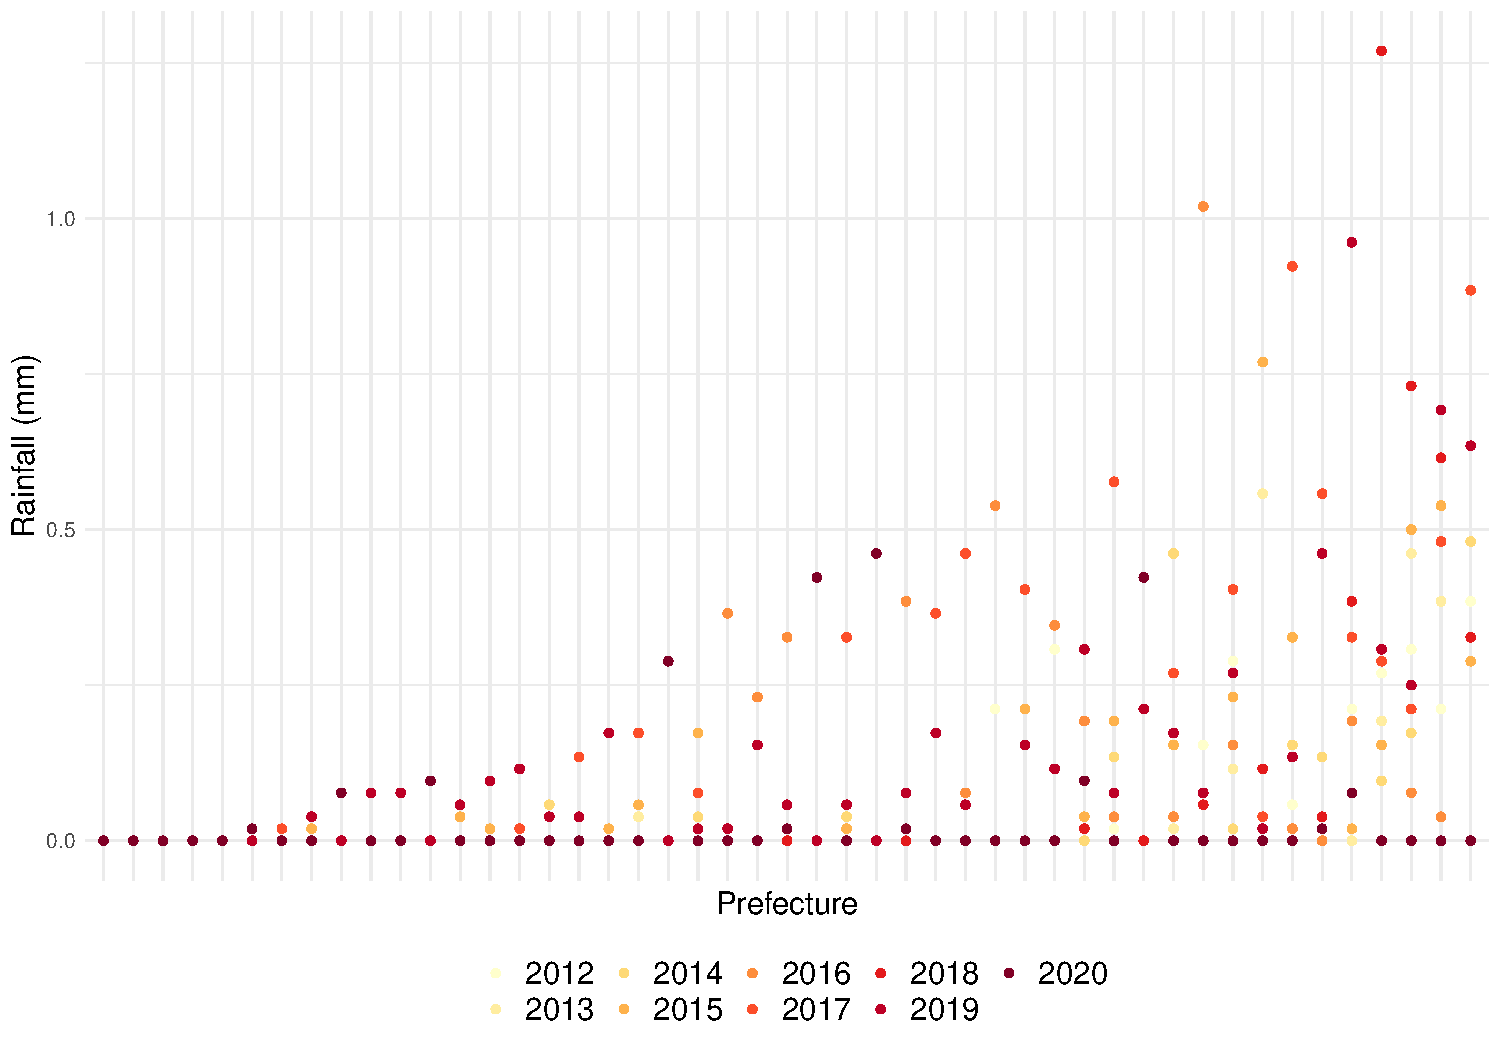
\includegraphics[width = 0.9\textwidth]{../Output/images/rainfall_diff.pdf}
  \label{fig:rainfall_diff}
  \footnotesize
  \begin{tablenotes}
    \item Notes:
      Rainfall (mm) at prefecture capitals between 6AM and 6PM on days of Center Test is used.
      Average across two test days in each year is shown in the figure.
      Prefectures positioned to the left on the x-axis are located at more northern parts of Japan.
  \end{tablenotes}
\end{figure}

\begin{figure}[H]
  \centering
  \caption{Average hourly snowfall (m) on two exam days in each prefecture each year}
  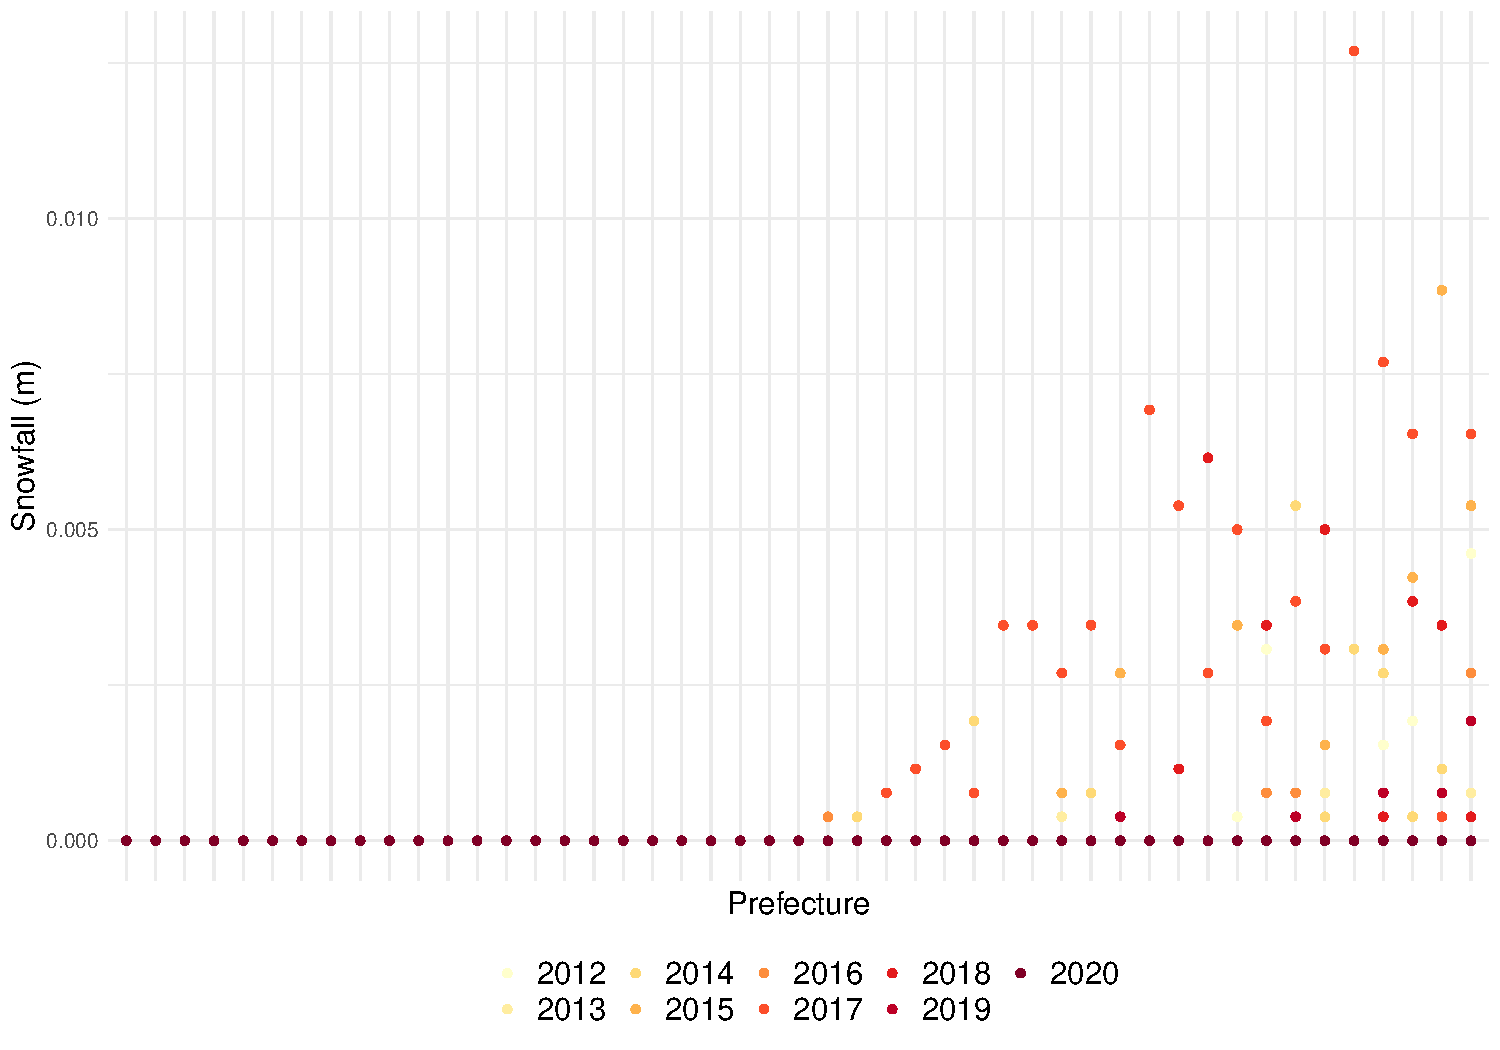
\includegraphics[width = 0.9\textwidth]{../Output/images/snowfall_diff.pdf}
  \label{fig:cum_snow_diff}
  \footnotesize
  \begin{tablenotes}
    \item Notes:
      Snowfall (m) at prefecture capitals between 6AM and 6PM on days of Center Test is used.
      Average across two test days in each year is shown in the figure.
      Prefectures positioned to the left on the x-axis are located at more northern parts of Japan.
  \end{tablenotes}
\end{figure}

\begin{figure}[H]
  \centering
  \caption{Average cumulated snow (m) on two exam days in each prefecture each year}
  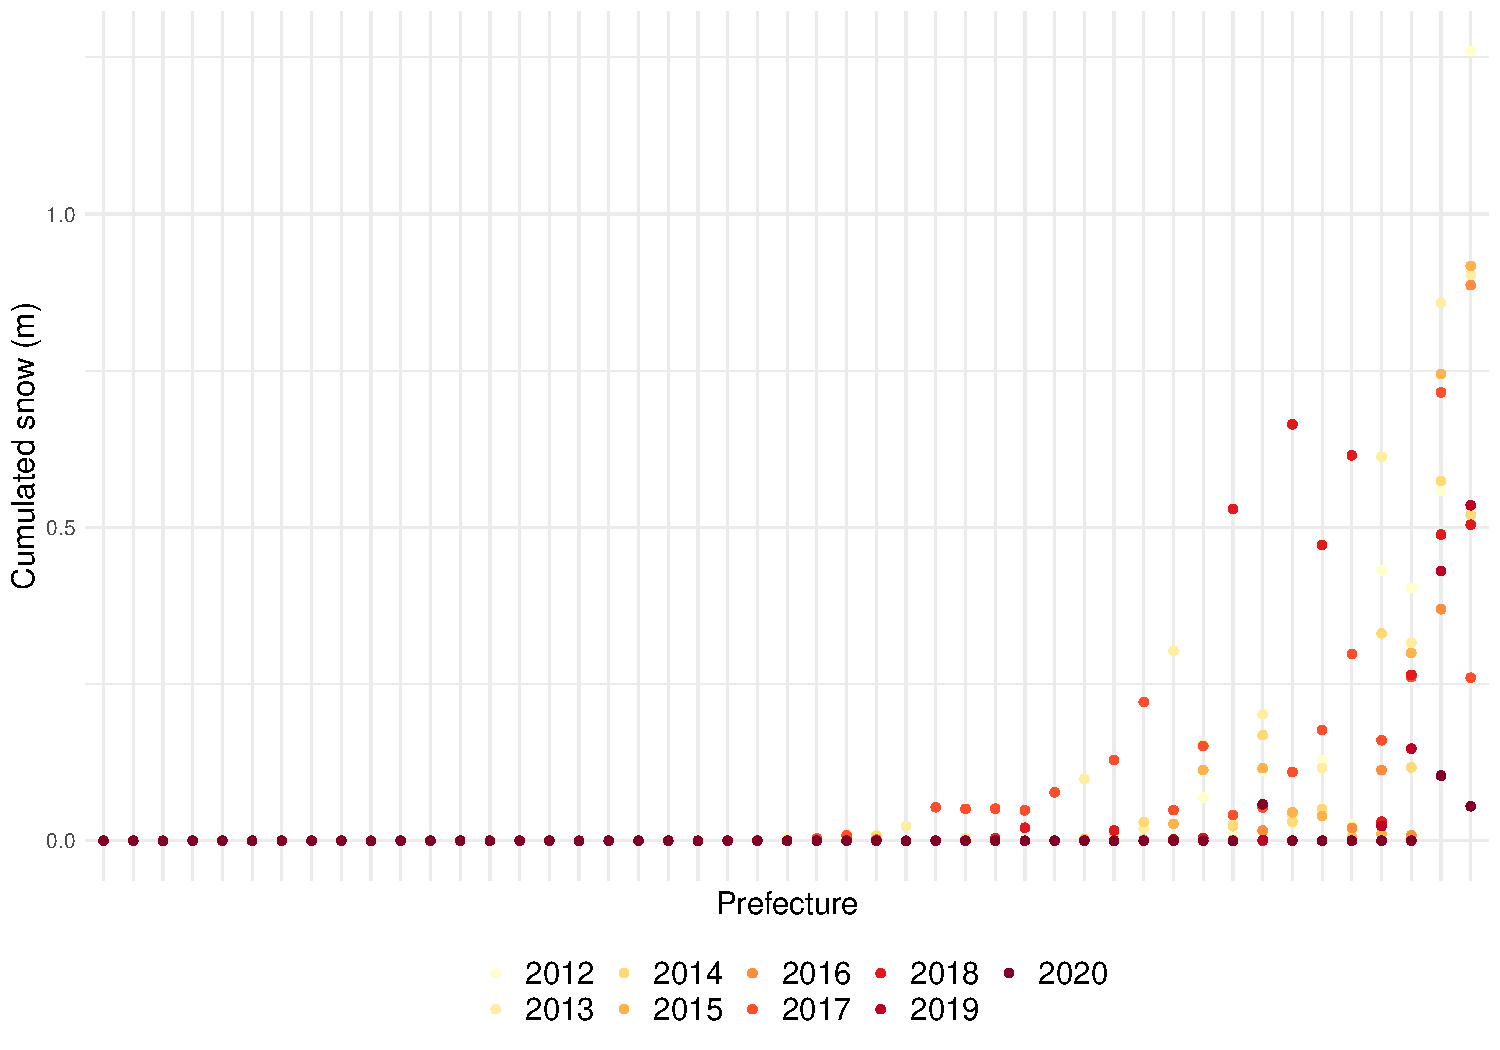
\includegraphics[width = 0.9\textwidth]{../Output/images/cum_snow_diff.pdf}
  \label{fig:cum_snow_diff}
  \footnotesize
  \begin{tablenotes}
    \item Notes:
      Cumulated snow (m) at prefecture capitals between 6AM and 6PM on days of Center Test is used.
      Average across two test days in each year is shown in the figure.
      Prefectures positioned to the left on the x-axis are located at more northern parts of Japan.
  \end{tablenotes}
\end{figure}

%\begin{figure}[H]
%  \centering
%  \caption{Map of average temperature on two exam days (average across years)}
%  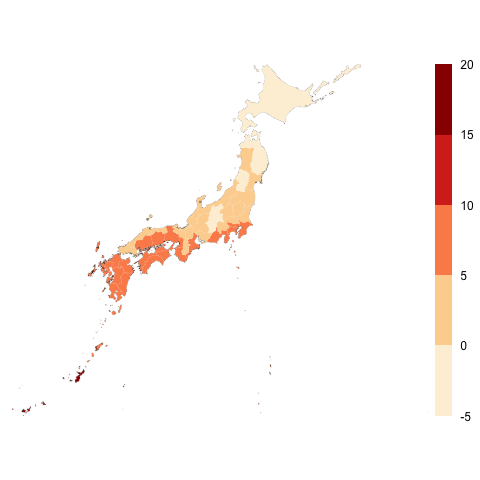
\includegraphics[width = 0.9\textwidth]{../Output/images/temperature_map.png}
%  \label{fig:temperature_map}
%  \footnotesize
%  \begin{tablenotes}
%    \item Notes:
%      Temperature at prefecture capitals between 6AM and 6PM on days of Center Test is used.
%      Average of the temperatures across years is shown in the map.
%  \end{tablenotes}
%\end{figure}
%
%\begin{figure}[H]
%  \centering
%  \caption{Map of average cumulated snow (m) on two exam days (average across years)}
%  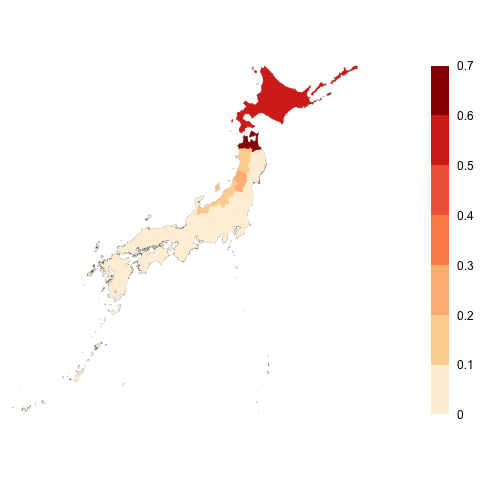
\includegraphics[width = 0.9\textwidth]{../Output/images/cum_snow_map.png}
%  \label{fig:cum_snow_map}
%  \footnotesize
%  \begin{tablenotes}
%    \item Notes:
%      Cumulated snow (m) on the ground at prefecture capitals between 6AM and 6PM on days of Center Test is used.
%      Average of the values across years is shown in the map.
%  \end{tablenotes}
%\end{figure}

\setcounter{figure}{0}
\setcounter{table}{0}
\renewcommand\thefigure{\Alph{section}.\arabic{figure}}
\renewcommand\thetable{\Alph{section}.\arabic{table}}
  
\section{Appendix tables}

\begin{table}[H]
  \center
  \caption{Regression: Admission share (\%) and average weather for 10 days before exam}
  
% Table created by stargazer v.5.2.2 by Marek Hlavac, Harvard University. E-mail: hlavac at fas.harvard.edu
% Date and time: Fri, Apr 02, 2021 - 13:40:23
\begin{tabular}{@{\extracolsep{5pt}}lcccc} 
\\[-1.8ex]\hline 
\hline \\[-1.8ex] 
 & \multicolumn{4}{c}{\textit{Dependent variable:}} \\ 
\cline{2-5} 
\\[-1.8ex] & \multicolumn{4}{c}{Matriculation share (\%)} \\ 
\\[-1.8ex] & (1) & (2) & (3) & (4)\\ 
\hline \\[-1.8ex] 
 Temperature (degree C) & $-$0.01 &  & $-$0.01 &  \\ 
  & (0.02) &  & (0.02) &  \\ 
  & & & & \\ 
 Temperature $\le$ 0 &  & $-$0.03 &  & 0.03 \\ 
  &  & (0.08) &  & (0.09) \\ 
  & & & & \\ 
 Temperature $>$ 0, $\le$ 3 &  & 0.03 &  & 0.05 \\ 
  &  & (0.05) &  & (0.05) \\ 
  & & & & \\ 
 Temperature $>$ 6, $\le$ 9 &  & 0.09 &  & 0.10 \\ 
  &  & (0.06) &  & (0.06) \\ 
  & & & & \\ 
 Temperature $>$ 9 &  & 0.001 &  & 0.02 \\ 
  &  & (0.11) &  & (0.11) \\ 
  & & & & \\ 
 Rainfall (mm) &  &  & $-$0.01 & $-$0.003 \\ 
  &  &  & (0.01) & (0.01) \\ 
  & & & & \\ 
 Snowfall (m) &  &  & $-$0.01 & $-$0.02 \\ 
  &  &  & (0.01) & (0.01) \\ 
  & & & & \\ 
 Cumulated snow (m) &  &  & $-$0.001 & $-$0.001 \\ 
  &  &  & (0.001) & (0.001) \\ 
  & & & & \\ 
\hline \\[-1.8ex] 
Prefecture FE & Yes & Yes & Yes & Yes \\ 
Year FE & Yes & Yes & Yes & Yes \\ 
Observations & 423 & 423 & 423 & 423 \\ 
\hline 
\hline \\[-1.8ex] 
\textit{Note:}  & \multicolumn{4}{r}{$^{*}$p$<$0.1; $^{**}$p$<$0.05; $^{***}$p$<$0.01} \\ 
\end{tabular} 

  \label{tab:reg_pre10}
  \small
  \begin{tablenotes}
    \item
      The outcome variable is the admission shares (\%) for the University of Tokyo from each prefecture.
      The admission share is calculated based on the ratio of the number of students from high schools in the prefecture to the total number of admission.
      I use average weather variables at prefecture capitals between 10 days before and 1 day before the first day of Center Test.
      Standard errors are clustered at the prefecture level.
  \end{tablenotes}
\end{table}

  
\end{document}



